\section{Results}\label{sec:results}

% \ra{1.1}
    {\begin{tabularx}{\textwidth}{lYYYYY} \toprule
         Copula/Asset & $t$ & Plackett & GMI & rotGumbel & NIG \\ \midrule
     \multicolumn{6}{l}{Individual Cryptos}                                                                                 \\
        \ \ \ BTC          & 73         & 4                 & 2                        & 1                  & 31                  \\
        \ \ \ ETH          & 3          & 6                 & 8                        & 94                 & 1                   \\
        \ \ \ ADA          & 0          & 0                 & 0                        & 0                  & 112                 \\
        \ \ \ LTC          & 13         & 0                 & 3                        & 32                 & 64                  \\
        \ \ \ XRP          & 0          & 31                & 3                        & 78                 & 0                   \\
   \multicolumn{6}{l}{Crypto Indices with BTC Constituent}                                                                  \\
        \ \ \ BITX         & 39         & 0                 & 14                       & 16                 & 12                  \\
        \ \ \ CRIX         & 47         & 0                 & 11                       & 3                  & 27                  \\
        \ \ \ BITW100      & 42         & 0                 & 8                        & 29                 & 2                   \\
    \multicolumn{6}{l}{Crypto Indices without BTC Constituent}                                                              \\
        \ \ \ BITW20       & 0          & 0                 & 0                        & 78                 & 3                   \\
        \ \ \ BITW70       & 0          & 0                 & 0                        & 80                 & 1                   \\
    \bottomrule
    \end{tabularx}
        \caption{Copula Selection Results. }










\subsection{Copula Selection Results}\label{sec: copula results}
The copula selection result is provides insight that help us understand the crypto market better, so
we illustrate the copula selection result in this section.
Decisions of the AIC procedure are summarised in table \ref{tab:copulasection}. \medskip

Overall, $t$-copula, rotated Gumbel (rotGumbel), and the NIG factor copula are the most frequently chosen copulae by the AIC procedure. \medskip

The $t$-copula is frequently chosen by AIC to model the dependency between the BTC and BTC involved indices, CRIX, BITX, BITW100, and the BTC future.
BTC and BTC involved indices exhibit strong tail dependence (both upper and lower tail) with BTCF.
We could interpret tail dependence much more of a tendency for one asset to be extreme when another is extreme and vice versa \citep{McNeil2015}.
In fact, the $t$ copula has been suggested in various empirical studies to model financial data, such as \cite{zeevi2002beyond} and \cite{breymann2003dependence}.
Those studies suggest $t$-copula is a better model over the Gaussian copula which financial data often seem to exhibit tail dependence. \medskip

On the other hand, the radially symmetric feature makes the $t$-copula not a good choice to model the other hedging pairs.
Demarta and McNeil describe the symmetry feature "strong", because if $(U_1, ..., U_d)$ is a vector distributed in $t$-copula,
then $(U_1, ..., U_d) \overset{\mathcal{L}}= (1-U_1, ..., 1-U_d)$.
This symmetry can be justified in the dependence structure between a future and its underlying by the theory of future pricing,
which suggests the price of a future is a function of the underlying price \citep{hull2003options}.
However, there is no such relationship between a future and an asset which is not the underlying, and so the radial symmetry becomes a drawback to model other hedging pairs e.g. ETH and BITX70.
Another drawback of the $t$-copula is the lack of flexibility to model off-diagonal region since Rho and nu jointly control the density of the off-diagonal region.
%The off-diagonal region (HF paper breymann2003dependence)
This is why sometimes the Gaussian Mix Independence (GMI) better model the dependence.  \medskip

Among the three popular copulae, rotGumbel copula shows its ability to model the dependency between ETH and BTCF,
94 out of 112 training sets are best fitted with the rotated Gumbel.
rotGumbel also performs well when modelling dependency between XRP, BITW20, BITW70, and the BTCF.
In particular, the whole time series of the two indices, BITW20 and BITW70, are best fitted solely with the rotated Gumbel copula.
The frequently chosen rotated Gumbel indicates the styled fact of financial data: prices tends to drop together.  \medskip
%  (ref) The reason for that

%The rotated Gumbel model the lower tail dependency very well, it has a lower quantile dependence controlled by its parameter

%BTC upper tail dependence BTC lower tail dependence (with fitted copula (t and rotGumbel) tail dependence)

%ETH upper tail dependence ETH lower tail dependence (with fitted copula (t and rotGumbel) tail dependence)

In fact, Clayton's AIC in many of the training sets is the second lowest, just higher than that of rotated Gumbel.
This is because the Clayton copula has the same ability to model the lower quantile dependence.
However, Clayton's radial like feature does not match the behaviour of the financial data. \medskip

It is worth to mention that although the NIG factor copula is penalised heavily due to its three parameters setup, it is frequently chosen to be the best copula to model the dependency between individual cryptos and the BTC future.
An extreme case would be ADA, only NIG factor is chosen in our dataset.
Another dependency structure being best described by the NIG factor copula is the pair of LTC-BTC future.
64 out of 112 training sets are best fitted by the NIG factor copula.
Indices like BITX and CRIX are sometimes best fitted with the NIG factor copula as well, accounting for modelling 12 and 27 training sets respectively.
The popularity of the NIG factor reflects the ability of the copula to model very complex dependency structure.
NIG factor copula is able to model the tail, radial asymmetry, and off diagonal behaviour.  \medskip %(ADA samples and fitted NIG samples)

Frank copula is generally not a good choice to model financial data just like what \cite{barbi2014copula} has reported.
Plackett is known for its dependence parameter can be written as the cross-product ratio \citep{joe1997multivariate}.
However, this feature does not bring the Plackett Copula advantage over other copulae to model the dependence structure between cryptos and BTCF. \medskip

\begin{table}[H]
 \ra{1.1}
    {\begin{tabularx}{\textwidth}{lYYYYY} \toprule
         Copula/Asset & $t$ & Plackett & GMI & rotGumbel & NIG \\ \midrule
     \multicolumn{6}{l}{Individual Cryptos}                                                                                 \\
        \ \ \ BTC          & 73         & 4                 & 2                        & 1                  & 31                  \\
        \ \ \ ETH          & 3          & 6                 & 8                        & 94                 & 1                   \\
        \ \ \ ADA          & 0          & 0                 & 0                        & 0                  & 112                 \\
        \ \ \ LTC          & 13         & 0                 & 3                        & 32                 & 64                  \\
        \ \ \ XRP          & 0          & 31                & 3                        & 78                 & 0                   \\
   \multicolumn{6}{l}{Crypto Indices with BTC Constituent}                                                                  \\
        \ \ \ BITX         & 39         & 0                 & 14                       & 16                 & 12                  \\
        \ \ \ CRIX         & 47         & 0                 & 11                       & 3                  & 27                  \\
        \ \ \ BITW100      & 42         & 0                 & 8                        & 29                 & 2                   \\
    \multicolumn{6}{l}{Crypto Indices without BTC Constituent}                                                              \\
        \ \ \ BITW20       & 0          & 0                 & 0                        & 78                 & 3                   \\
        \ \ \ BITW70       & 0          & 0                 & 0                        & 80                 & 1                   \\
    \bottomrule
    \end{tabularx}
        \caption{Copula Selection Results. }









\label{tab:copulasection}}
\end{table}

\subsection{Hedging Effectiveness Results}\label {sec: HE results}
In this section, we analyse the out-of-sample hedging effectiveness (HE) of BTCF as hedging.
HE is defined as $$\text{HE} = 1-\frac{\rho_h}{\rho_s},$$
a measure of the percentage reduction of portfolio risk attribute, in our case the spot $\rho_s$,
to hedged portfolio risk attribute $\rho_h$.
A higher HE indicates a higher hedging effectiveness and larger risk reduction. \medskip

The HE above is a generalisation of Ederington measure of hedging performance, where we,
in addition to variance, include other risk measures: Expected Shortfall 5\% and 1\% (ES5 and ES1), Value-at-Risk 5\% and 1\% (VaR5 and VaR1), and ERM.
In particular, ES5 is recommended by the Basel Committee on Banking Supervision (BCBS) to replace VaR as a quantitative risk metrics system.
The proposed reform aimed at enhancing the risk metric system's ability to capture tail risk. \medskip
%Discussions of the issue can be found in literatures.
%
We obtain a time series of out-of-sample $r^h$ of each hedging pair and each risk reduction objective by concatenating the out-of-sample results.
Then, we apply stationary block bootstrapping (SB) to the time series introduced by \cite{Politis1994} in our analysis in order to preserve the temporal structure of the data while sampling.
The SB procedure is as follow.
Assume a time series with $N$ observations $\{X_t\}_{t \in [1,N]}$ is a strong stationary, weakly dependence time series of interest,
we form blocks of samples $B = \{X_i, ..., X_{i+j-1}\}$.
Index $i$ is a random variable uniformly distributed over $[1,2,...,N]$ and $j$ is geometric distributed random variable with parameter .
The block index $i$ and block length $j$ are independent.
For any index $k$ which is greater than $N$, the sample $X_k$ is defined to be $X_{k(\mod N)}$.
For each block, we calculate the hedging effectiveness with different risk measures mentioned above.
We choose p=0.005, implying the expected block length is 200.
100 blocks are drawn for each risk minimising objective and spot. \medskip

From figure \ref{fig:HEboxplot}, we can see, as expected, the BTC involving spots, the BTC, CRIX, BITX and BITW100, are well hedged by the BTCF.
Surprisingly, the performances are consistent across different risk reduction objectives and different HE evaluation.
The median HE to BTC generated by various risk reduction objectives is ranging from 89.45\% to 99.31\%, median HE to CRIX is ranging from 81.13\% to 95.22\%,
median HE to BITX is ranging from 79.06\% to 94.84\%, median HE to BITW100 Is ranging from 71.07\% to 92.98\%. \medskip

The HE of BTCF to other cryptos and indices are substantially lower than to the BTC involving spots, but the consistency the performances across different risk reduction objectives and HE evaluation remains.
The median HE to BITW20 generated by various risk reduction objectives is ranging from 24.67\% to 47.02\%, median HE to BITW70 is ranging from 23.61\% to 49.30\%,
median HE to ADA is ranging from 9.01\% to 29.30\%, median HE to ETH Is ranging from 30.07\% to 36.18\%, median HE to LTC Is ranging from 37.74\% to 51.30\%,
median HE to XRP Is ranging from 0.46\% to 30.89\%.
\begin{figure}[h]
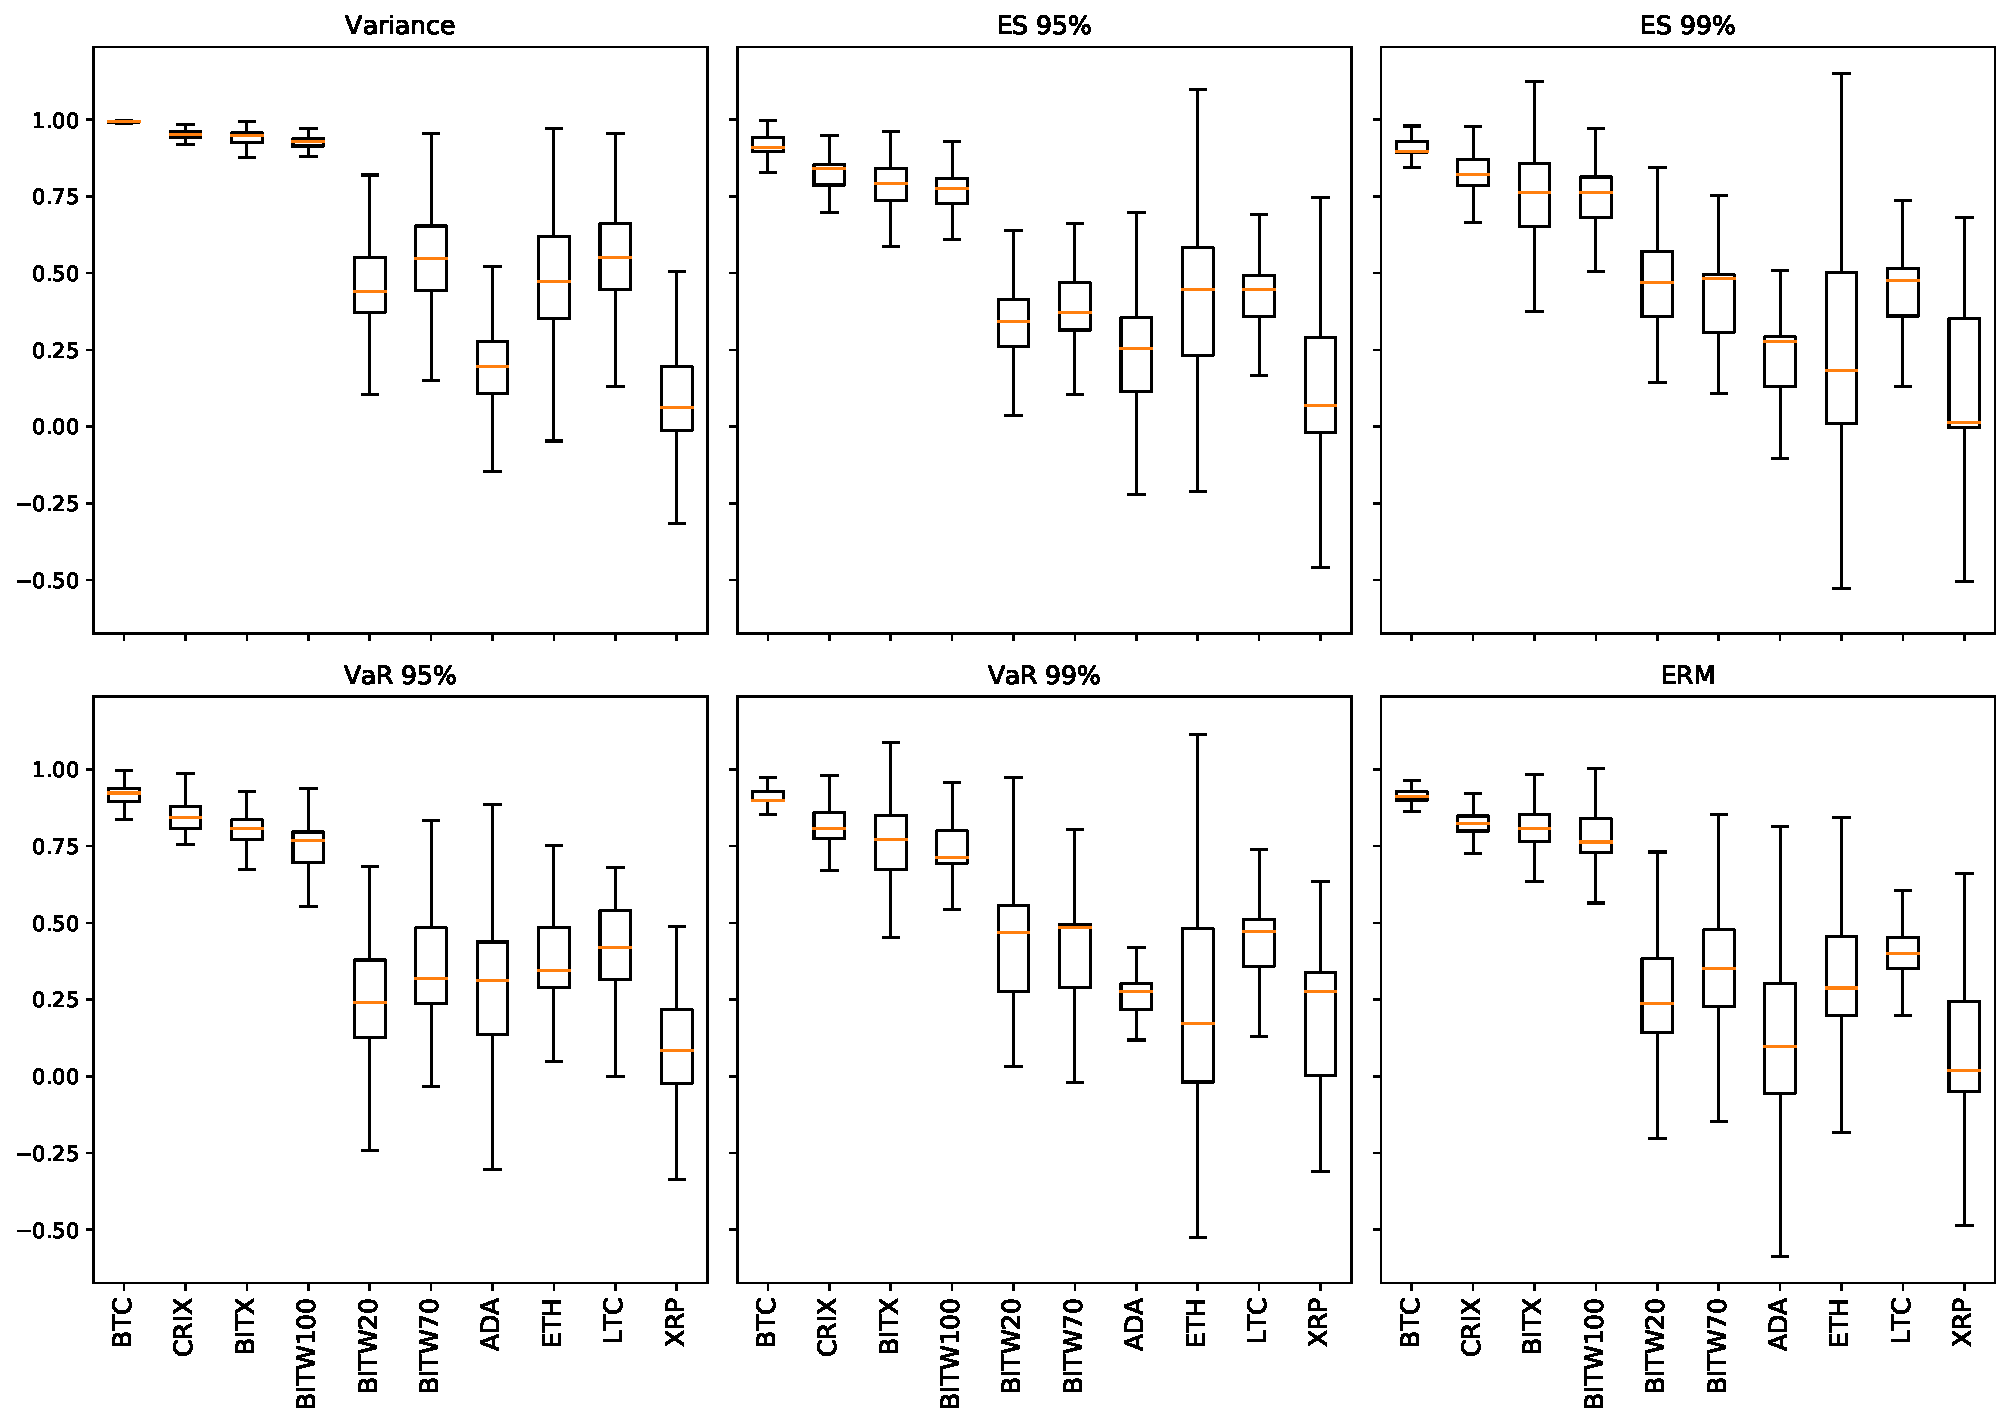
\includegraphics[width=\textwidth]{_pics/ES5_HE_boxplot.pdf}
  \caption{HE evaluated in different risk measures to various assets generated by minimizing ES5.
  \href{http://www.quantlet.com/}{\includegraphics[width=20pt]{_pics/qletlogo_tr.png}} }
\label{fig:HEboxplot}
\end{figure}
